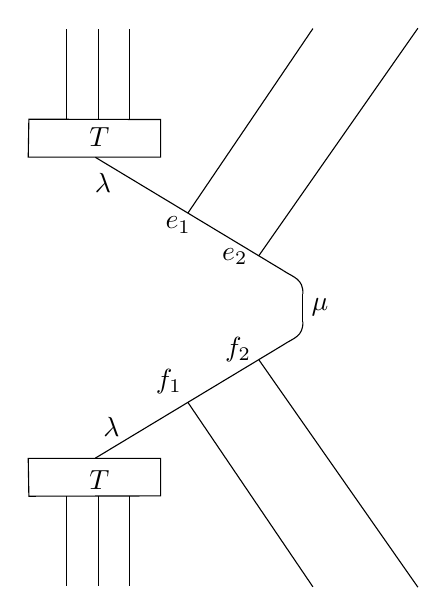
\begin{tikzpicture}[yscale=-1,scale=0.04,baseline={([yshift=-.5ex]current bounding box.center)}]
\begin{scope}[shift={(0.00mm,719.29mm)}]
% path id='path4136'
% path spec='m 175.82745,-431.55186 -2.0203,120.20815 420.22346,0 0,-119.198 z'
\draw [fill=none,draw=black] (175.83mm,-431.55mm)
-- ++(-2.02mm,120.21mm)
-- ++(420.22mm,0.00mm)
-- ++(0.00mm,-119.20mm)
-- cycle
;
% path id='path4138'
% path spec='m 295.62951,-431.55186 0,-285.31477'
\draw [fill=none,draw=black] (295.63mm,-431.55mm)
-- ++(0.00mm,-285.31mm)
;
% path id='path4140'
% path spec='m 395.62951,-431.55186 0,-285.31477'
\draw [fill=none,draw=black] (395.63mm,-431.55mm)
-- ++(0.00mm,-285.31mm)
;
% path id='path4142'
% path spec='m 495.62951,-431.55186 0,-285.31477'
\draw [fill=none,draw=black] (495.63mm,-431.55mm)
-- ++(0.00mm,-285.31mm)
;
% path id='path4152'
% path spec='M 387.14286,-310.49492 983.54317,48.955407'
\draw [fill=none,draw=black] (387.14mm,-310.49mm)
-- (983.54mm,48.96mm)
;
% path id='path4154'
% path spec='m 983.42722,49.064995 c 34.77508,22.656028 63.18648,26.055305 62.70548,73.875365'
\draw [fill=none,draw=black] (983.43mm,49.06mm)
.. controls ++(34.78mm,22.66mm) and ++(0.48mm,-47.82mm) .. ++(62.71mm,73.88mm)
;
% path id='path4156'
% path spec='m 175.82745,765.63068 -2.0203,-120.20815 420.22346,0 0,119.198 z'
\draw [fill=none,draw=black] (175.83mm,765.63mm)
-- ++(-2.02mm,-120.21mm)
-- ++(420.22mm,0.00mm)
-- ++(0.00mm,119.20mm)
-- cycle
;
% path id='path4158'
% path spec='m 295.62951,765.63068 0,285.31472'
\draw [fill=none,draw=black] (295.63mm,765.63mm)
-- ++(0.00mm,285.31mm)
;
% path id='path4160'
% path spec='m 395.62951,765.63068 0,285.31472'
\draw [fill=none,draw=black] (395.63mm,765.63mm)
-- ++(0.00mm,285.31mm)
;
% path id='path4162'
% path spec='m 495.62951,765.63068 0,285.31472'
\draw [fill=none,draw=black] (495.63mm,765.63mm)
-- ++(0.00mm,285.31mm)
;
% path id='path4164'
% path spec='M 387.14286,644.57374 983.54317,285.12339'
\draw [fill=none,draw=black] (387.14mm,644.57mm)
-- (983.54mm,285.12mm)
;
% path id='path4166'
% path spec='m 983.42722,285.0138 c 34.77508,-22.65604 63.18648,-26.05532 62.70548,-73.87538'
\draw [fill=none,draw=black] (983.43mm,285.01mm)
.. controls ++(34.78mm,-22.66mm) and ++(0.48mm,47.82mm) .. ++(62.71mm,-73.88mm)
;
% path id='path4168'
% path spec='m 1046.1392,122.76934 0,88.51462'
\draw [fill=none,draw=black] (1046.14mm,122.77mm)
-- ++(0.00mm,88.51mm)
;
% path id='path4170'
% path spec='M 680.84282,-133.55686 1077.8328,-719.44534'
\draw [fill=none,draw=black] (680.84mm,-133.56mm)
-- (1077.83mm,-719.45mm)
;
% path id='path4172'
% path spec='M 906.10683,1.80358 1411.1831,-720.45549'
\draw [fill=none,draw=black] (906.11mm,1.80mm)
-- (1411.18mm,-720.46mm)
;
% path id='path4174'
% path spec='M 680.84282,467.66259 1077.8328,1053.5511'
\draw [fill=none,draw=black] (680.84mm,467.66mm)
-- (1077.83mm,1053.55mm)
;
% path id='path4176'
% path spec='M 906.10683,332.30214 1411.1831,1054.5612'
\draw [fill=none,draw=black] (906.11mm,332.30mm)
-- (1411.18mm,1054.56mm)
;
\node [black] at (411.43mm,-230.49mm) { $\lambda$ };
\node [black] at (650.00mm,-95.64mm) { $e_1$ };
\node [black] at (830.00mm,4.36mm) { $e_2$ };
\node [black] at (620.00mm,400.36mm) { $f_1$ };
\node [black] at (840.00mm,300.36mm) { $f_2$ };
\node [black] at (1100.00mm,164.36mm) { $\mu$ };
\node [black] at (438.00mm,546.36mm) { $\lambda$ };
\node [black] at (400mm,-375.64mm) { $T$ };
\node [black] at (400mm,714.36mm) { $T$ };
\end{scope}
\end{tikzpicture}
